\chapter{Конструкторская часть}
В данной части работы будет рассмотрен псевдокод линейного и бинарного алгоритмов поиска.

\section{Псевдокоды рассматриваемых алгоритмов}

В листингах~\ref{alg:bin_search}--\ref{alg:lin_search} рассмотрены псевдокоды алгоритмов поиска, входными данными для них являются:
\begin{enumerate}
	\item $a$~---~массив;
	\item $N$~---~число элементов в массиве;
	\item $x$~---~искомое число.
\end{enumerate}

Программа должна вернуть индекс искомого элемента в массиве, если он в нем присутствует, или $-1$~---~в противном случае. Оператор $\gets$~обозначает присваивание значение переменной, оператор $[i]$ обозначает получение элемента из массива с индексом $i$, рассматривается только целочисленное деление. Иные операторы подобны математическим.
\begin{algorithm}
\caption{Псевдокод алгоритма бинарного поиска.}\label{alg:bin_search}
\begin{algorithmic}
	\Require {Элементы в массиве упорядочены по неубыванию.}
	\State {$left_i \gets 0$}
	\State {$right_i \gets N - 1$}
	\State {$middle_i \gets (left_i + right_i)/2$}
	\While {$array[middle_i] != target \land left_i \leq right_i$}
		\If {$array[middle_i] < target$}
			\State {$left_i \gets middle_i + 1$}
		\Else
			\State {$right_i \gets middle_i - 1$}
		\EndIf
		\State {$middle_i \gets (left_i + right_i)/2$}
	\EndWhile
	\If {$left_i > right_i$}
		\State \Return {$-1$}
	\Else
		\State \Return {$middle_i$}
	\EndIf
\end{algorithmic}
\end{algorithm}

\begin{algorithm}
\caption{Псевдокод алгоритма линейного поиска.}\label{alg:lin_search}
\begin{algorithmic}
	\For{$i$ от $1$ до $N-1$}
		\If {$array[i] = target$}
			\State \Return {$i$}
		\EndIf
	\EndFor
	\State \Return {$-1$}
\end{algorithmic}
\end{algorithm}


\section{Алгоритмы}

На рисунках \ref{img:binSearch1} и \ref{img:binSearch2} представлена схема алгоритма бинарного поиска.
\includeimage
{binSearch1}
{f}
{H}
{1\textwidth}
{Алгоритм бинарного поиска, часть 1}

\includeimage
{binSearch2}
{f}
{H}
{1\textwidth}
{Алгоритм бинарного поиска, часть 2}

На рисунке \ref{fig:dummySearch} представлена схема алгоритма поиска полным перебором.


\begin{figure}[H]
	\centering
	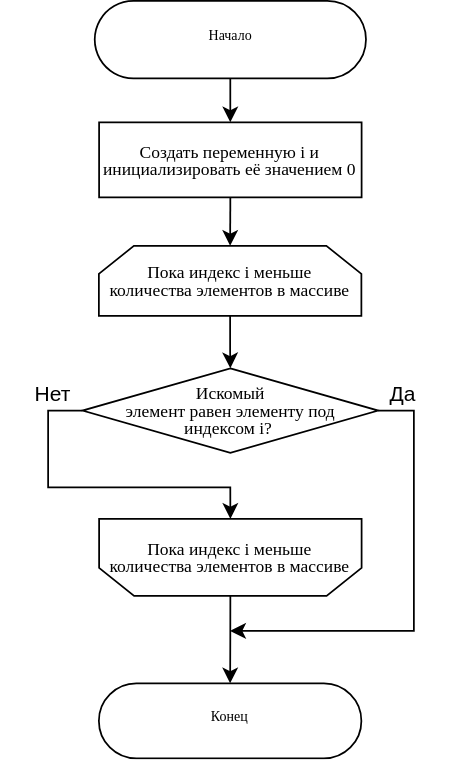
\includegraphics[width=0.75\textwidth]{inc/img/dummySearch.pdf}
	\caption{Алгоритм поиска полным перебором}
	\label{fig:dummySearch}
\end{figure}

\section*{Вывод}
В данной части работы был написан псевдокод для алгоритмов линейного и бинарного поиска, а также представлены схемы этих алгоритмов.








